\section{mr::hemisphere\-Sampler Class Reference}
\label{classmr_1_1hemisphereSampler}\index{mr::hemisphereSampler@{mr::hemisphereSampler}}
Sample a full or partial hemisphere around a direction.  


{\tt \#include $<$mr\-Sampler.h$>$}

Inheritance diagram for mr::hemisphere\-Sampler::\begin{figure}[H]
\begin{center}
\leavevmode
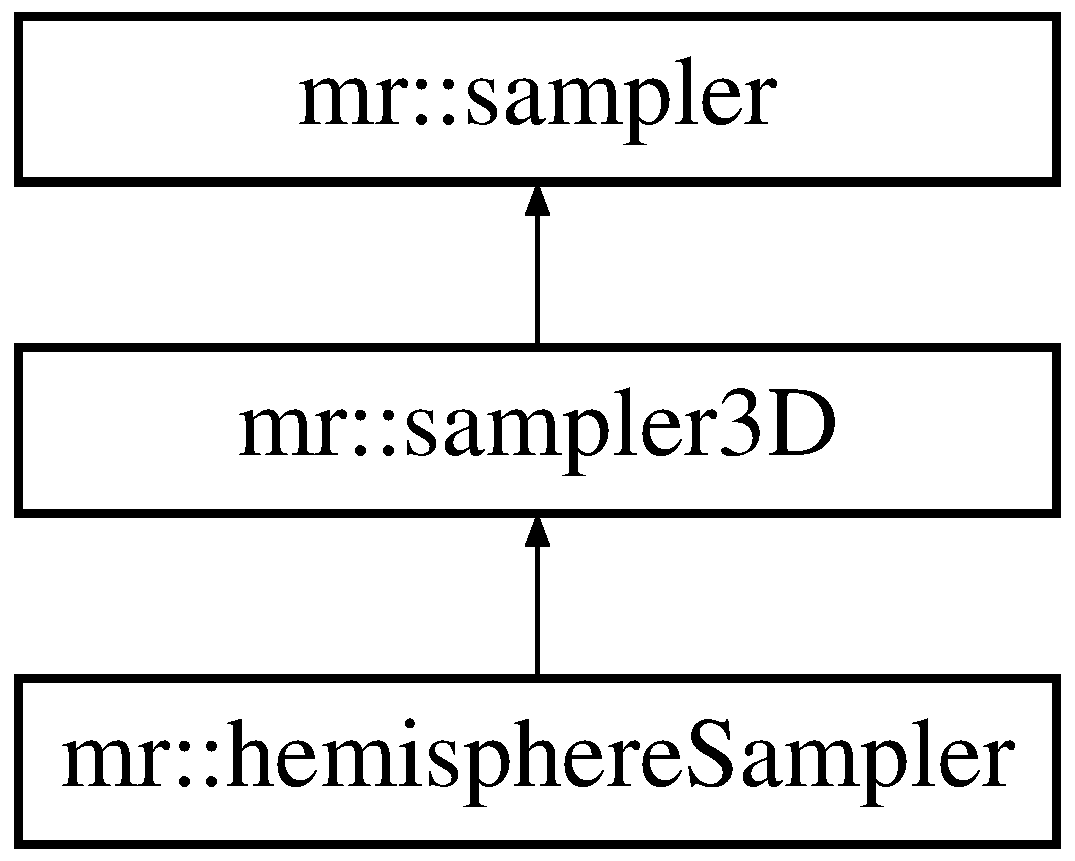
\includegraphics[height=3cm]{classmr_1_1hemisphereSampler}
\end{center}
\end{figure}
\subsection*{Public Member Functions}
\begin{CompactItemize}
\item 
{\bf hemisphere\-Sampler} (const mi\-Vector \&Nin)
\item 
{\bf hemisphere\-Sampler} (const mi\-Vector \&Nin, const mi\-Uint \&num\-Samples)
\item 
{\bf $\sim$hemisphere\-Sampler} ()
\item 
bool {\bf uniform} (const mi\-State $\ast$const state)
\item 
bool {\bf cosine} (const mi\-State $\ast$const state)
\item 
bool {\bf uniform} (const mi\-State $\ast$const state, const mi\-Scalar max)
\item 
bool {\bf cosine} (const mi\-State $\ast$const state, const mi\-Scalar max)
\item 
const mi\-Scalar {\bf weight} ()
\end{CompactItemize}
\subsection*{Protected Member Functions}
\begin{CompactItemize}
\item 
void {\bf UVNframe} ()
\item 
void {\bf cosine\-Distribution} ()
\item 
void {\bf cosine\-Distribution} (const mi\-Scalar max)
\item 
void {\bf uniform\-Distribution} ()
\item 
void {\bf uniform\-Distribution} (const mi\-Scalar max)
\item 
void {\bf calculate\-Direction} ()
\end{CompactItemize}


\subsection{Detailed Description}
Sample a full or partial hemisphere around a direction. 



\subsection{Constructor \& Destructor Documentation}
\index{mr::hemisphereSampler@{mr::hemisphere\-Sampler}!hemisphereSampler@{hemisphereSampler}}
\index{hemisphereSampler@{hemisphereSampler}!mr::hemisphereSampler@{mr::hemisphere\-Sampler}}
\subsubsection{\setlength{\rightskip}{0pt plus 5cm}mr::hemisphere\-Sampler::hemisphere\-Sampler (const mi\-Vector \& {\em Nin})\hspace{0.3cm}{\tt  [inline]}}\label{classmr_1_1hemisphereSampler_a0}


Constructor. Nin is the direction to sample around. sphere\-Percent is percentage of sphere to cover. This call is to be used when sampling adaptively (ie. the number of samples to be taken are not known or may vary, or you may exit the loop early). \index{mr::hemisphereSampler@{mr::hemisphere\-Sampler}!hemisphereSampler@{hemisphereSampler}}
\index{hemisphereSampler@{hemisphereSampler}!mr::hemisphereSampler@{mr::hemisphere\-Sampler}}
\subsubsection{\setlength{\rightskip}{0pt plus 5cm}mr::hemisphere\-Sampler::hemisphere\-Sampler (const mi\-Vector \& {\em Nin}, const mi\-Uint \& {\em num\-Samples})\hspace{0.3cm}{\tt  [inline]}}\label{classmr_1_1hemisphereSampler_a1}


Constructor. Nin is the direction to sample around. sphere\-Percent is percentage of sphere to cover. num\-Samples is the number of samples to take. It HAS to be mi\-Uint\& \index{mr::hemisphereSampler@{mr::hemisphere\-Sampler}!~hemisphereSampler@{$\sim$hemisphereSampler}}
\index{~hemisphereSampler@{$\sim$hemisphereSampler}!mr::hemisphereSampler@{mr::hemisphere\-Sampler}}
\subsubsection{\setlength{\rightskip}{0pt plus 5cm}mr::hemisphere\-Sampler::$\sim${\bf hemisphere\-Sampler} ()\hspace{0.3cm}{\tt  [inline]}}\label{classmr_1_1hemisphereSampler_a2}




\subsection{Member Function Documentation}
\index{mr::hemisphereSampler@{mr::hemisphere\-Sampler}!calculateDirection@{calculateDirection}}
\index{calculateDirection@{calculateDirection}!mr::hemisphereSampler@{mr::hemisphere\-Sampler}}
\subsubsection{\setlength{\rightskip}{0pt plus 5cm}void mr::hemisphere\-Sampler::calculate\-Direction ()\hspace{0.3cm}{\tt  [inline, protected]}}\label{classmr_1_1hemisphereSampler_b5}


\index{mr::hemisphereSampler@{mr::hemisphere\-Sampler}!cosine@{cosine}}
\index{cosine@{cosine}!mr::hemisphereSampler@{mr::hemisphere\-Sampler}}
\subsubsection{\setlength{\rightskip}{0pt plus 5cm}bool mr::hemisphere\-Sampler::cosine (const mi\-State $\ast$const {\em state}, const mi\-Scalar {\em max})\hspace{0.3cm}{\tt  [inline]}}\label{classmr_1_1hemisphereSampler_a6}


Get one sample using a cosine distribution over the max angle (expressed as a cosine [0,1]) or return false. \index{mr::hemisphereSampler@{mr::hemisphere\-Sampler}!cosine@{cosine}}
\index{cosine@{cosine}!mr::hemisphereSampler@{mr::hemisphere\-Sampler}}
\subsubsection{\setlength{\rightskip}{0pt plus 5cm}bool mr::hemisphere\-Sampler::cosine (const mi\-State $\ast$const {\em state})\hspace{0.3cm}{\tt  [inline]}}\label{classmr_1_1hemisphereSampler_a4}


Get one sample using a cosine distribution over the whole hemisphere or return false. \index{mr::hemisphereSampler@{mr::hemisphere\-Sampler}!cosineDistribution@{cosineDistribution}}
\index{cosineDistribution@{cosineDistribution}!mr::hemisphereSampler@{mr::hemisphere\-Sampler}}
\subsubsection{\setlength{\rightskip}{0pt plus 5cm}void mr::hemisphere\-Sampler::cosine\-Distribution (const mi\-Scalar {\em max})\hspace{0.3cm}{\tt  [inline, protected]}}\label{classmr_1_1hemisphereSampler_b2}


\index{mr::hemisphereSampler@{mr::hemisphere\-Sampler}!cosineDistribution@{cosineDistribution}}
\index{cosineDistribution@{cosineDistribution}!mr::hemisphereSampler@{mr::hemisphere\-Sampler}}
\subsubsection{\setlength{\rightskip}{0pt plus 5cm}void mr::hemisphere\-Sampler::cosine\-Distribution ()\hspace{0.3cm}{\tt  [inline, protected]}}\label{classmr_1_1hemisphereSampler_b1}


\index{mr::hemisphereSampler@{mr::hemisphere\-Sampler}!uniform@{uniform}}
\index{uniform@{uniform}!mr::hemisphereSampler@{mr::hemisphere\-Sampler}}
\subsubsection{\setlength{\rightskip}{0pt plus 5cm}bool mr::hemisphere\-Sampler::uniform (const mi\-State $\ast$const {\em state}, const mi\-Scalar {\em max})\hspace{0.3cm}{\tt  [inline]}}\label{classmr_1_1hemisphereSampler_a5}


Get one sample using a uniform distribution over the max angle (expressed as a cosine [0,1]) or return false. \index{mr::hemisphereSampler@{mr::hemisphere\-Sampler}!uniform@{uniform}}
\index{uniform@{uniform}!mr::hemisphereSampler@{mr::hemisphere\-Sampler}}
\subsubsection{\setlength{\rightskip}{0pt plus 5cm}bool mr::hemisphere\-Sampler::uniform (const mi\-State $\ast$const {\em state})\hspace{0.3cm}{\tt  [inline]}}\label{classmr_1_1hemisphereSampler_a3}


Get one sample using a uniform distribution over the whole hemisphere or return false. \index{mr::hemisphereSampler@{mr::hemisphere\-Sampler}!uniformDistribution@{uniformDistribution}}
\index{uniformDistribution@{uniformDistribution}!mr::hemisphereSampler@{mr::hemisphere\-Sampler}}
\subsubsection{\setlength{\rightskip}{0pt plus 5cm}void mr::hemisphere\-Sampler::uniform\-Distribution (const mi\-Scalar {\em max})\hspace{0.3cm}{\tt  [inline, protected]}}\label{classmr_1_1hemisphereSampler_b4}


\index{mr::hemisphereSampler@{mr::hemisphere\-Sampler}!uniformDistribution@{uniformDistribution}}
\index{uniformDistribution@{uniformDistribution}!mr::hemisphereSampler@{mr::hemisphere\-Sampler}}
\subsubsection{\setlength{\rightskip}{0pt plus 5cm}void mr::hemisphere\-Sampler::uniform\-Distribution ()\hspace{0.3cm}{\tt  [inline, protected]}}\label{classmr_1_1hemisphereSampler_b3}


\index{mr::hemisphereSampler@{mr::hemisphere\-Sampler}!UVNframe@{UVNframe}}
\index{UVNframe@{UVNframe}!mr::hemisphereSampler@{mr::hemisphere\-Sampler}}
\subsubsection{\setlength{\rightskip}{0pt plus 5cm}void mr::hemisphere\-Sampler::UVNframe ()\hspace{0.3cm}{\tt  [inline, protected]}}\label{classmr_1_1hemisphereSampler_b0}


\index{mr::hemisphereSampler@{mr::hemisphere\-Sampler}!weight@{weight}}
\index{weight@{weight}!mr::hemisphereSampler@{mr::hemisphere\-Sampler}}
\subsubsection{\setlength{\rightskip}{0pt plus 5cm}const mi\-Scalar mr::hemisphere\-Sampler::weight ()\hspace{0.3cm}{\tt  [inline]}}\label{classmr_1_1hemisphereSampler_a7}


This returns a weight (dot product) of the sample with respect to the original Nin vector. Useful in uniform distributions only. 

The documentation for this class was generated from the following file:\begin{CompactItemize}
\item 
{\bf mr\-Sampler.h}\end{CompactItemize}
